%!TEX TS-program = xelatex
%!TEX encoding = UTF-8 Unicode
% !TEX root = ../../metm.tex

\section{Filtri Digitali}

% dal computer music tutorial
Gli esperimenti sull'implementazione digitale dei filtri risalgono ai primi anni 50.
Diverse fasi di sviluppo matematico e concettuale hanno permesso solo dagli anni 60
una vera teorizzazione e semplice implementazione. Solo dagli anni 80 sono stati
possibili implementazioni in tempo reale per un utilizzo musicale.

\begin{quote}
  Un filtro digitale è un processo di calcolo o un algoritmo attraverso il quale
  un segnale digitale o una sequenza di numeri (la sequenza di entrata) è
  trasformata in una seconda sequenza di numeri denominata segnale digitale di
  uscita.\footnote{Rabiner 1972.}
\end{quote}

In questo senso quindi ogni strumento digitale con un'entrata ed un'uscita è un
filtro digitale. Comunemente l'uso del termine \emph{filtro} descrive un dispositivo
in grado di amplificare o attenuare porzioni di spettro. Ma anche riverberi e linee
di ritardo sono filtri, questo dovrebbe suggerirci l'idea che un filtro può
modificare lo spettro di un segnale entrante, ma anche la sua struttura temporale,
sia su una scala molto piccola che su una molto ampia e che quindi struttura
spettrale e struttura temporale di un segnale sono in relazione diretta tra loro.

Un'equazione di un filtro digitale non necessariamente rivela le sue caratteristiche
audio. In letteratura un filtro è rappresentato attraverso la \tz.
La \tz~ mappa gli effetti dei ritardi del campione in un'immagine
bidimensionale del dominio della frequenza denominato \emph{piano complesso zeta}.
Su questo piano vengono rappresenntati \emph{poli} per i picchi di risonanza e
\emph{zeri} per i punti di ampiezza nulla dell'uscita del filtro. Un \emph{filtro
a due poli}, per esempio, indica due picchi di risonanza.

esempio due poli

La \tz~è un concetto importante per lo sviluppo di un filtro in quanto rappresentazione
matematica di passaggio tra le caratteristiche del filtro ed i suoi parametri di
implementazione. Rimane però un'applicazione astratta con relazioni solo indirette
con i parametri fisici del filtro.

Nella rappresentazione software di un filtro si opera in processi applicati
ai campioni audio, in termini di operazioni matematiche e ritardi a questi applicati.
Generalmente quindi si descrive un filtro con diagrammi di flusso che ne dichiarino
il percorso, rispopste all'impulso e risposte in frequenza.

\subsection{Risposte all'impulso, in frequenza e in fase.}

Si può osservare l'effetto di un filtro sia nel dominio del tempo che in quello
della frequenza. Un'immagine \emph{prima} ed una \emph{dopo} l'applicazione, possono
mostrare l'effetto del filtro. Senza dubbio alcune tipologie di segnali d'entrata
possono mostrare l'effetto del filtro più chiaramente di altre. Per testare un
filtro abbiamo bisogno di un segnale di entrata contenente tutte le frequenze necessarie.

Il \rb, che contiene tutte le frequenze ci indica come un filtro risponde nel dominio
della frequenza. Ma una visione completa dell'azione del filtro deve contemplare
un'analisi anche nel dominio del tempo, nella sua risposta ad i transienti temporali.

Esiste una relazione inversa tra durata e contenuto spettrale di un segnale.
Un'oscillazione sinusoidale di infinita durata contiene una sola frequenza, un
impulso ha uno spettro allargato.

Nei sistemi digitali il segnale più breve possibile è di un solo campione. Questo
segnale continee energia su tutto lo spettro di frequenze ad una data frequenza
di campionamento.

Una via generalizzata di caratterizzare un filtro è appunto quella di descriverne
il comportamento temporale in risposta ad un impulso unitario, di un solo campione.
La sua uscita, la risposta all'impulso, descrive il comportamento in ampiezza nel
tempo in uscita dal filtro, in perfetta coerennza con quanto descrivibile nel dominio
della frequenza. Lo stesso segnale di uscita descritto in domini diversi.

In linea generale un IR lungo corrisponde ad una banda molto stretta in frequenza,
mentre un impulso corto ad una risposta larga in frequenza.

Un'ulteriore caratteristica dei filtri è l'eventuale effetto sulla fase di un
segnale sinusoidale in entrata. La risposta in fase di un filtro può essere descritta
in termini di rotazione di fase espressa in radianti oppure in termini di ritardo
di fase, che ne indica lo slittamento temporale in secondi.

\subsection{Filtri come equazioni}

Un filtro digitale può essere espresso anche mediante un'equazione che metta in
relaizone il segnale d'entrata con quello d'uscita. Il segnale d'uscita può essere
descritto come risultato del lavoro di somme, sottrazioni e moltiplicazioni del
campione corrente o di quelli precedentemete transitati.
% Questo tipo di equazioni si chiama \emph{equazione differenziale lineare}.

In letteratura sul \emph{signal processing} il segnale in entrata ad un filtro si
chiama $ x $ mentre la sua uscita si chiama $ y $. I campioni in entrata, processati
ed in uscita dal filtro vengono convenzionalmente numerati, indicizzati ed indicati
($ x[0] $ è il campione zero del segnale entrante, $ x[1] $ il suo successivo
$ n+1 $ mentre $ y[1] $ è lo stesso campione in uscita).

\subsection{Simple Lowpass Filter}

Un semplice filtro passa basso opera una media tra il campione attuale ed il suo
precedente in entrata. In altri termini, opera una somma tra il campione attuale
ed il precedente e poi divide per due. Osservandolo matematicamente, un filtro di
questo tipo potrebbe essere denominato interpolatore, o mediatore, di due
campioni adiacenti. Dato che una rapida variazione d'ampiezza tra due campioni
adiacenti è osservabile solo in presenza di alte frequenze, un filtro interpolatore
come quello appena descritto tenderà a ridurre le differenze tra i campioni,
interpolando, e quindi attenuando le componenti ad alta frequenza in uscita.

\begin{figure}[ht]
  \centering
  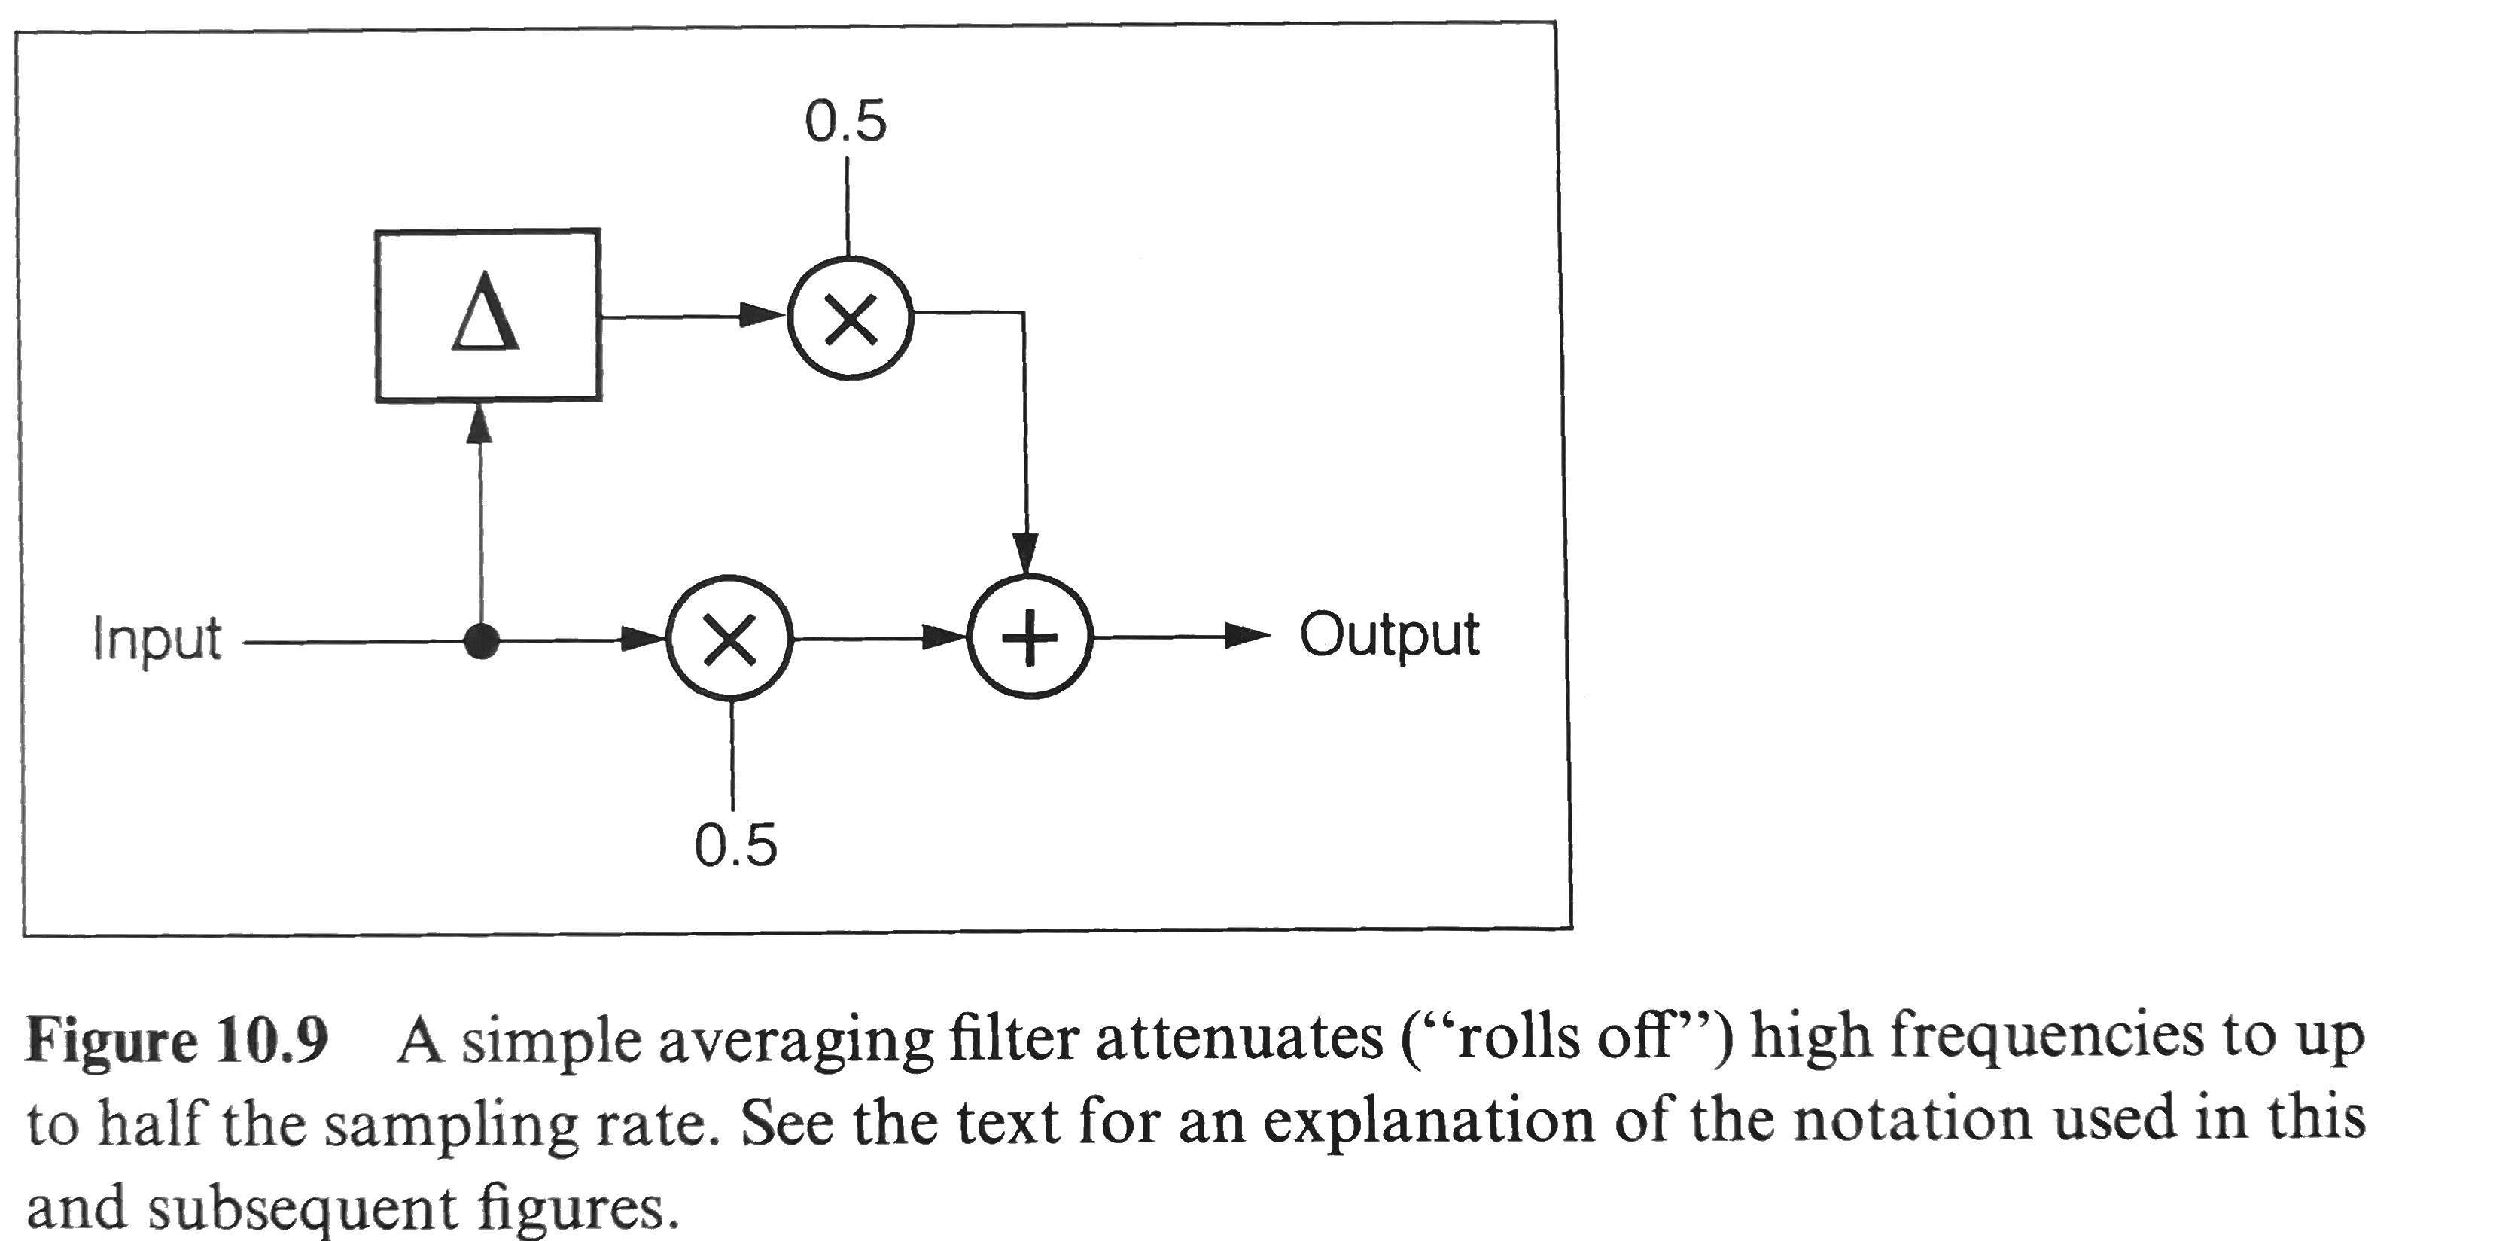
\includegraphics[width=\textwidth]{CAPITOLI/0500/IMG/CT_Lowpass.pdf}
  \caption[]{Lowpass. Computer Music Tutorial.}
  \label{CT-Lowpass}
\end{figure}

L'equazione di un filtro di questo tipo è la sequente:

\begin{equation}
  \label{lowpass}
  y[n] = (0.5 \times x[n]) + (0.5 \times x[n-1])
\end{equation}

dove $y[n]$ è il segnale d'uscita, $(0.5 \times x[n])$ è la metà del campione in
entrata e $(0.5 \times x[n-1])$ è la metà del campione precedente.

La costante di riscalamento ($0.5$) nell'espressione è denominata \emph{coefficiente
del filtro}.

L'equazione trascritta in linguaggio Faust:

\lstinputlisting{CAPITOLI/0500/CODES/lowpass.dsp}

produce il diagramma di flusso:

\begin{figure}[ht]
  \centering
  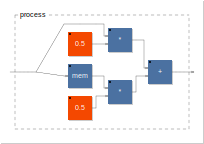
\includegraphics[]{CAPITOLI/0500/CODES/lowpass-svg/process}
  \caption[]{Lowpass. Faust Diagram.}
  \label{fdlowpass}
\end{figure}

Questa la risposta all'impulso:

\lstinputlisting{CAPITOLI/0500/CODES/lowpass.txt}

\clearpage
